% task3.tex — Deep Anomaly Detection and Data Representation

\section{DEEP ANOMALY DETECTION AND DATA REPRESENTATION} \label{sec:task3}

This section explores deep learning and dimensionality reduction approaches for anomaly detection: autoencoder-based reconstruction error thresholding, autoencoder bottleneck embeddings with OC-SVM, and PCA-based dimensionality reduction with OC-SVM.

% --- Autoencoder Architecture ---
\subsection{Autoencoder Architecture and Training} \label{sec:autoencoder}

    We designed a symmetric autoencoder with the following architecture:
    \begin{itemize}
        \item \textbf{Encoder:} Input (51) $\rightarrow$ 128 $\rightarrow$ 64 $\rightarrow$ 16 (bottleneck), with BatchNorm, ReLU, and Dropout (0.2) after each h layer.
        \item \textbf{Decoder:} 16 $\rightarrow$ 64 $\rightarrow$ 128 $\rightarrow$ 51 (reconstruction), with a symmetric architecture.
    \end{itemize}

    \noindent
    Since the feature space contains both numerical and categorical (one-hot encoded) features, we used a \textbf{composite loss function}: MSE for numerical features and Cross-Entropy for each categorical feature.
    This ensures the autoencoder learns appropriate reconstruction objectives for each feature type.
    The model was trained exclusively on the \textbf{normal data} from the training partition (10,758 samples) in a semi-supervised way: by learning to reconstruct only normal traffic, anomalies should produce higher reconstruction errors due to unfamiliar feature patterns.

% --- Hyperparameter Tuning ---
\subsection{Hyperparameter Tuning} \label{sec:hp_tuning}

    We performed a grid search over learning rates $\{5 \times 10^{-3},\, 10^{-3},\, 5 \times 10^{-4},\, 10^{-4}\}$ with a maximum of 150 epochs and early stopping (patience = 15).

    % \begin{table}[H]
    %     \centering
    %     \begin{tabular}{@{}lccc@{}}
    %         \toprule
    %         \textbf{Learning Rate} & \textbf{Min Val Loss} & \textbf{Best Epoch} & \textbf{Early Stop?} \\
    %         \midrule
    %         $5 \times 10^{-3}$            & 0.2160 & 26  & Yes (epoch 41) \\
    %         $1 \times 10^{-3}$            & 0.1232 & 78  & Yes (epoch 93) \\
    %         $\mathbf{5 \times 10^{-4}}$   & \textbf{0.1140} & \textbf{82} & Yes (epoch 97) \\
    %         $1 \times 10^{-4}$            & 0.1609 & 148 & No \\
    %         \bottomrule
    %     \end{tabular}
    %     \vspace{0.5em}
    %     \caption{Learning rate grid search results (bottleneck dimension = 16).}
    %     \label{tab:lr_search}
    % \end{table}

    \vspace{-0.2cm}

    \begin{figure}[H]
        \centering
        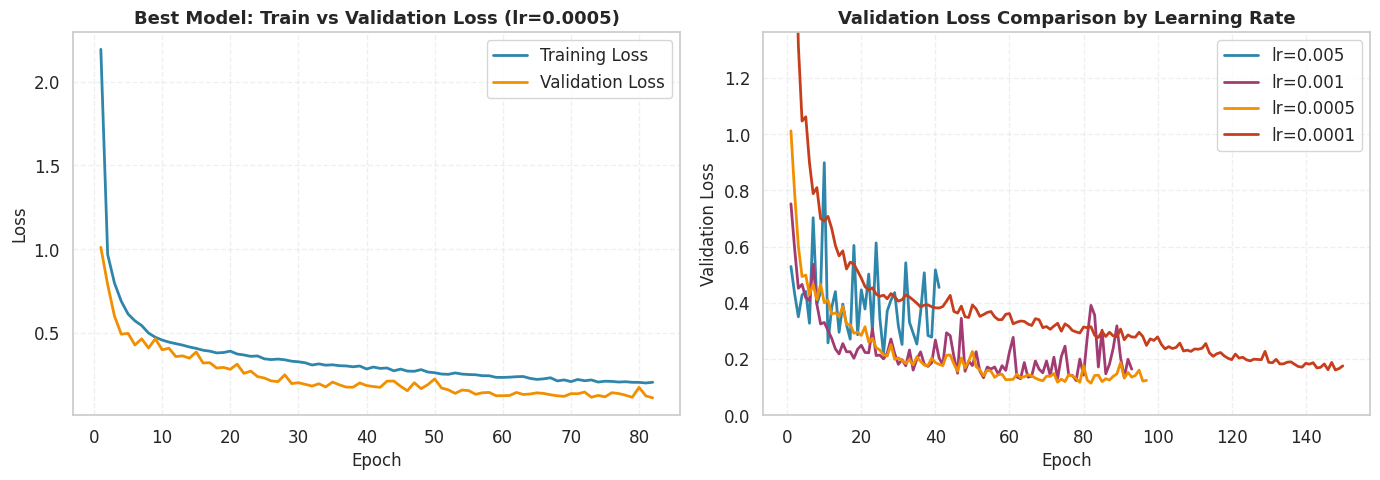
\includegraphics[width=\linewidth]{images/task3/task3_autoencoder_analysis_combined.png}
        \vspace{-0.4cm}
        \caption{AE validation loss curves across four learning rates (right) and train and val curves for the best model (left).}
        \label{fig:task3_ae_loss}
    \end{figure}

    \vspace{-0.2cm}

    \noindent
    The learning rate $5 \times 10^{-4}$ achieves the lowest validation loss (0.1140) with a stable convergence.
    Higher learning rates converge faster but to worse optima due to instability in the early training phase, while $10^{-4}$ reaches an higher minimum and slower convergence.

% --- Reconstruction Error Threshold ---
\subsection{Reconstruction Error Analysis} \label{sec:reconstruction}

    We computed the Empirical Cumulative Distribution Function (ECDF) of reconstruction errors on the autoencoder validation partition containing normal traffic only. 
    An analysis of the underlying error statistics justified this choice: while the distribution possesses a tight core ($\text{Median} = 0.0117$ and $\text{Mean} = 0.1140$), it exhibits a heavy right tail stretching to an absolute maximum error of $44.7958$. 
    This confirms that a small subset of normal traffic generates high reconstruction errors, likely due to variations in traffic patterns or slight model misspecification. 
    Consequently, the 95th percentile was selected as the operational anomaly threshold: $\theta = 0.3604$. 
    This design choice explicitly establishes a baseline False Positive Rate (FPR) of approximately 5\% on pure normal traffic, balancing detection sensitivity against the operational costs of false alarms.

    % This threshold choice is visually supported by the localized ECDF in Figure~\ref{fig:task3_combined_plots}(a), which flattens dramatically past an error of $1.0$ as it enters the extreme outlier tail. 
    % When evaluating the multi-partition ECDF comparison in Figure~\ref{fig:task3_combined_plots}(b), distinct rightward shifts across the curves validate the model's operational logic. 
    % While the normal-only validation set saturates at 95\% below $\theta$, the full training set shifts rightward, crossing the threshold line at approximately 71\% on the Y-axis. 
    % This matches expectations, as the remaining 29\% of samples above the threshold reflect the known anomaly contamination the model fails to reconstruct. 
    % Similarly, the test set shifts furthest to the right, crossing the threshold at roughly 32\% on the Y-axis; this aligns with its high 63\% anomaly density and confirms that unseen attack vectors are successfully pushed into high-error regions. \\
    
    This threshold choice is visually supported by Figure~\ref{fig:task3_combined_plots} (a), where the validation ECDF flattens past $1.0$ as it enters the outlier tail. 
    In Figure~\ref{fig:task3_combined_plots} (b), clear rightward shifts validate the model's logic: while the normal-only validation set has 95\% of samples below $\theta$, the training set crosses the threshold at 71\%, reflecting the 29\% anomaly contamination. 
    The test set shifts furthest to the right, crossing the threshold at approximately 32\%, which aligns with its 63\% anomaly density and confirms that unseen attack signatures produce high reconstruction errors.

    % \begin{figure}[H]
    %     \centering
    %     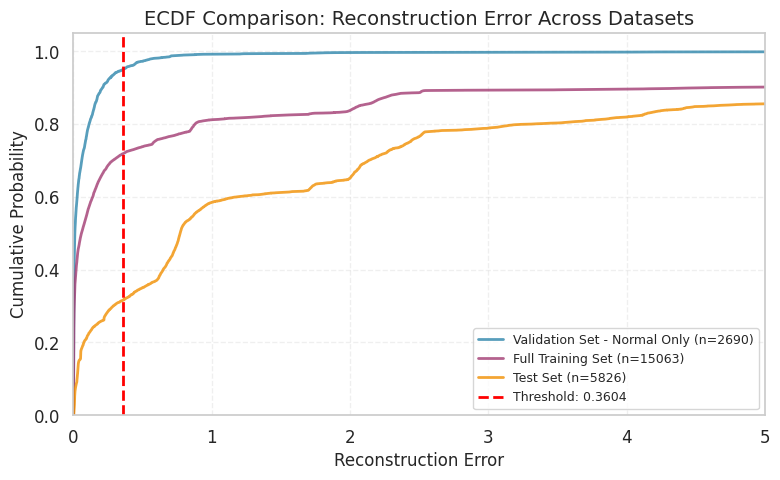
\includegraphics[width=0.6\linewidth]{images/task3/task3_ecdf_combined.png}
    %     \caption{ECDF of reconstruction errors across Validation (normal only), full Training, and Test sets. The rightward shift of the Training and Test curves confirms that the autoencoder successfully learned the normal manifold: anomalous samples produce substantially higher reconstruction errors.}
    %     \label{fig:task3_ecdf}
    % \end{figure}

    \begin{figure}[]
        \centering
        \begin{subfigure}[b]{0.49\linewidth}
            \centering
            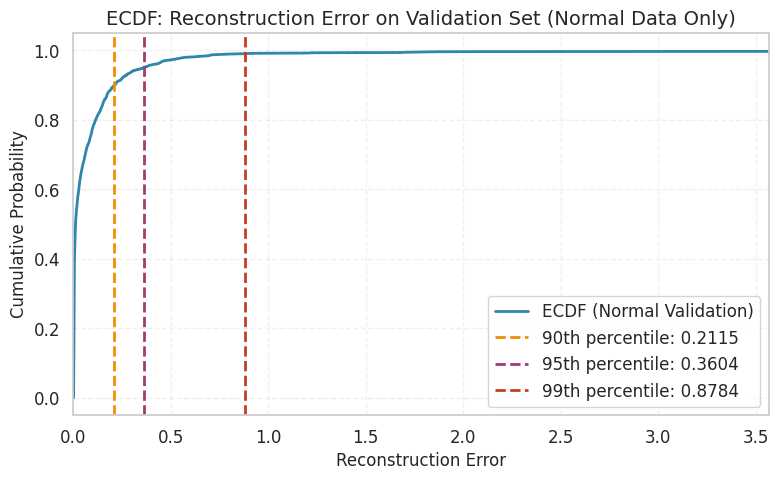
\includegraphics[width=\linewidth]{images/task3/task3_ecdf_treshold.png}
            \label{fig:ae_threshold_selection}
        \end{subfigure}
        \hfill
        \begin{subfigure}[b]{0.49\linewidth}
            \centering
            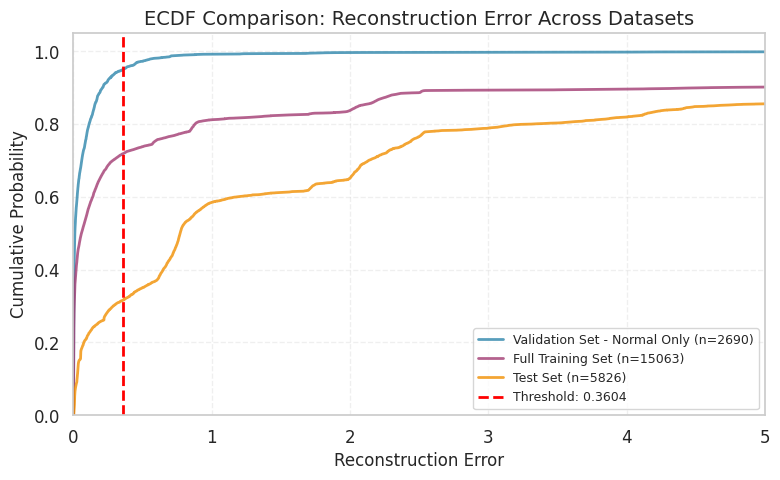
\includegraphics[width=\linewidth]{images/task3/task3_ecdf_combined.png}
            \label{fig:ae_ecdf_comparison}
        \end{subfigure}
        \vspace{-0.3cm}
        \caption{Empirical Cumulative Distribution Function (ECDF) analysis of Autoencoder reconstruction errors. Figure~(a) shows the localized threshold selection on the normal-only Validation split, highlighting candidate percentiles. Figure~(b) demonstrates the structural rightward shift of the anomaly-laden Training and Test curves relative to the clean validation manifold.}
        \label{fig:task3_combined_plots}
    \end{figure}

    \vspace{-0.2cm}

    \noindent
    Samples with a reconstruction error exceeding $\theta$ are classified as anomalies. As shown in Table~\ref{tab:ae_reconstruction}, the model achieves a test F1-Macro of \textbf{0.7547}, demonstrating strong generalization and confirming the efficacy of the learned normal traffic manifold. 
    Note that performance metrics on the Validation Set in Table~\ref{tab:ae_reconstruction} utilize the full 3,767-sample stratified validation partition (which includes anomalies) to evaluate threshold efficacy. In contrast, the autoencoder's weights were trained, and the threshold $\theta$ itself was selected, using exclusively the 2,690 normal-traffic samples within that partition.

    \vspace{-0.1cm}

    \begin{table}[H]
        \centering
        \begin{tabular}{@{}lccc@{}}
            \toprule
            \textbf{Dataset} & \textbf{F1-Macro} & \textbf{Precision (Anomaly)} & \textbf{Recall (Anomaly)} \\
            \midrule
            Train Set      & 0.9132 & 0.8823 & 0.8690 \\
            Validation Set & 0.9024 & 0.8713 & 0.8487 \\
            Test Set       & \textbf{0.7547} & 0.7994 & 0.8669 \\
            \bottomrule
        \end{tabular}
        \vspace{0.5em}
        \caption{Autoencoder reconstruction error anomaly detection ($\theta = 0.3604$).}
        \label{tab:ae_reconstruction}
    \end{table}

\vspace{-0.2cm}

% --- Bottleneck + OC-SVM ---
\subsection{Latent Space Anomaly Detection (AE + OC-SVM)} \label{sec:bottleneck}

    We extracted the 16-dimensional bottleneck embeddings from the trained encoder and used them as input features for an OC-SVM trained on normal data only.
    We tested two values of $\nu$: 0.01 (conservative) and 0.1.
    The choice of $\nu = 0.1$ was empirically motivated: the ECDF of reconstruction errors for normal samples in the bottleneck space shows a roughly 10th-percentile inflection, suggesting that approximately 10\% of normal points inhabit atypical regions of the compressed manifold.
    Setting $\nu$ below this fraction forces the OC-SVM to exclude geometrically valid normal points, shrinking the boundary and inflating false positives.

    \begin{table}[H]
        \centering
        \begin{minipage}{0.48\linewidth}
            \centering
            \resizebox{0.75\linewidth}{!}{%
                \begin{tabular}{@{}lcc@{}}
                    \toprule
                    \textbf{$\nu$} & \textbf{Train F1-Macro} & \textbf{Test F1-Macro} \\
                    \midrule
                    0.01         & 0.7662 & 0.6645 \\
                    \textbf{0.1} & \textbf{0.8300} & \textbf{0.7795} \\
                    \bottomrule
                \end{tabular}%
            }
            \vspace{0.5em}
            \caption{AE Bottleneck + OC-SVM: impact of $\nu$ on performance.}
            \label{tab:bottleneck_nu}
        \end{minipage}\hfill
        \begin{minipage}{0.48\linewidth}
            \centering
            \resizebox{\linewidth}{!}{%
                \begin{tabular}{@{}lccc@{}}
                    \toprule
                    \textbf{Dataset Partition} & \textbf{Precision} & \textbf{Recall} & \textbf{F1-Macro} \\
                    \midrule
                    Train Set            & 0.7529             & 0.7628          & 0.8300 \\
                    Validation Set       & 0.7588             & 0.7391          & 0.8250 \\
                    Test Set             & \textbf{0.8168}    & \textbf{0.8821} & \textbf{0.7795} \\
                    \bottomrule
                \end{tabular}%
            }
            \vspace{0.5em}
            \caption{Performance metrics for the optimal AE Bottleneck + OC-SVM configuration ($\nu=0.1$).}
            \label{tab:bottleneck_perf}
        \end{minipage}
    \end{table}

    \vspace{-0.2cm}

    \noindent
    The $\nu = 0.1$ configuration yields a substantial \textbf{+11.5 percentage points} improvement on the test set compared to the $\nu=0.01$ baseline, making AE Bottleneck + OC-SVM the \textbf{best-performing method overall} (test F1-Macro = 0.7795).
    This improvement occurs because the conservative $\nu = 0.01$ is too restrictive in the compressed 16-dimensional latent space, where normal traffic embeddings exhibit greater relative dispersion and require a looser boundary to capture legitimate variations.
    By allowing this wider boundary, the optimal model achieves an exceptional anomaly recall of \textbf{88.21\%} while maintaining a strong precision of \textbf{81.68\%}, demonstrating that non-linear feature compression effectively isolates structural anomalies while mitigating the risk of alert fatigue.

% --- PCA + OC-SVM ---
\subsection{PCA-based Anomaly Detection} \label{sec:pca}

    % As a linear baseline for dimensionality reduction, we applied PCA on normal training data and selected \textbf{20 components}, capturing 95.5\% of cumulative explained variance.
    % An OC-SVM ($\nu = 0.01$) was then trained on the PCA-transformed normal data.

    As a linear baseline for dimensionality reduction, we applied Principal Component Analysis (PCA) strictly on the normal training data. 
    Analyzing the cumulative explained variance allowed us to determine the optimal sub-space projection; as illustrated in Figure~\ref{fig:task3_pca_elbow}, an explicit elbow point emerges at \textbf{20 components}, capturing exactly 95.5\% of the total dataset variance. 
    This confirms the significant feature redundancy mathematically identified in our earlier correlation analysis (\Cref{sec:correlation}). 
    By reducing the input space from 51 to 20 dimensions, we achieve a substantial \textbf{60\% dimensionality reduction} while retaining the vast majority of information. 
    An OC-SVM ($\nu = 0.01$) was subsequently trained on this optimized linear sub-space.

    \begin{figure}[H]
        \centering
        \begin{minipage}{0.48\linewidth}
            \centering
            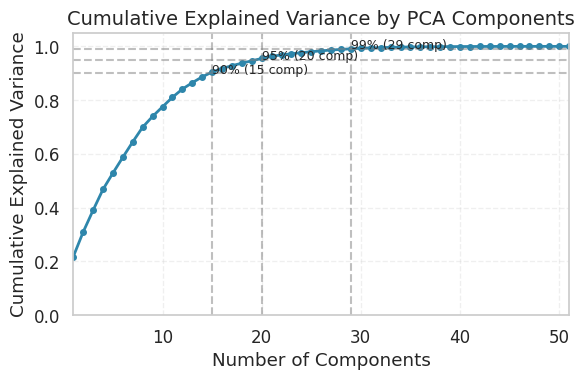
\includegraphics[width=\linewidth]{images/task3/task3_pca_explained_variance.png}
            \caption{Cumulative explained variance vs.\ number of PCA components (fitted on normal training data only). The elbow at 20 components (95.5\% cumulative variance) guides our selection.}
            \label{fig:task3_pca_elbow}
        \end{minipage}\hfill
        \begin{minipage}{0.48\linewidth}
            \centering
            \makeatletter\def\@captype{table}\makeatother
            \resizebox{\linewidth}{!}{%
                \begin{tabular}{@{}lccc@{}}
                    \toprule
                    \textbf{Dataset} & \textbf{F1-Macro} & \textbf{Precision (A)} & \textbf{Recall (A)} \\
                    \midrule
                    Train Set        & 0.8835 & 0.9655 & 0.7206 \\
                    Validation Set   & 0.8664 & 0.9548 & 0.6862 \\
                    Test Set         & \textbf{0.7377} & \textbf{0.8533} & \textbf{0.7186} \\  
                    \bottomrule
                \end{tabular}%
            }
            \vspace{0.5em}
            \caption{PCA + OC-SVM performance (20 components).}
            \label{tab:pca_ocsvm}
        \end{minipage}
    \end{figure}

    % PCA + OC-SVM achieves a test F1-Macro of 0.7377, nearly matching the original full-dimensional OC-SVM (0.7477) despite a \textbf{60\% dimensionality reduction} ($51 \to 20$).
    % This confirms the significant feature redundancy identified in the correlation analysis (\Cref{sec:correlation}), and establishes that the primary relationships in this dataset are largely linear.

    The PCA + OC-SVM pipeline achieves a final test F1-Macro of 0.7377 (Table~\ref{tab:pca_ocsvm}), nearly matching our full-dimensional raw baseline (0.7477) despite working with less than half the features. 
    This confirms that the primary macro-relationships within the dataset are largely linear. 

    However, the test partition reveals a distinct performance asymmetry: the model maintains high anomaly precision (\textbf{85.33\%}) but struggles with a more moderate recall (\textbf{71.86\%}). 
    While the linear PCA transformation effectively isolates prominent outliers, it strips away the subtle, non-linear interactions required to flag stealthy attack variants. 
    This linear bottleneck explains why the non-linear feature extraction performed by the Autoencoder (Section~\ref{sec:bottleneck}) achieves a significantly higher anomaly recall (\textbf{88.21\%}).

% --- Comprehensive Comparison ---
\subsection{Comprehensive Method Comparison} \label{sec:comparison_task3}

    Table~\ref{tab:method_comparison_f1} aggregates the final performance across all evaluated models on the test partition.

    \begin{table}[H]
        \centering
        \resizebox{\linewidth}{!}{%
            \begin{tabular}{@{}lccccc@{}}
                \toprule
                \textbf{Anomaly Detection Method} & \textbf{Train F1-Macro} & \textbf{Test F1-Macro} & \textbf{Test Precision (A)} & \textbf{Test Recall (A)} \\
                \midrule
                Original OC-SVM ($\nu = 0.05$)    & 0.9026                  & 0.7477                 & 0.8084                            & 0.8258                         \\
                PCA + OC-SVM ($\nu = 0.01$)       & 0.8835                  & 0.7377                 & \textbf{0.8533}                   & 0.7186                         \\
                AE Reconstruction Error           & 0.9132                  & 0.7547                 & 0.7994                            & 0.8669                         \\
                \textbf{AE Bottleneck + OC-SVM} ($\nu = 0.1$) & 0.8300      & \textbf{0.7795}        & 0.8168                            & \textbf{0.8821}                \\
                \bottomrule
            \end{tabular}%
        }
        \vspace{0.5em}
        \caption{Comprehensive comparison of anomaly detection methods across metrics.}
        \label{tab:method_comparison_f1}
    \end{table}

    \noindent
    The \textbf{AE Bottleneck + OC-SVM} achieves the highest test F1-Macro (\textbf{0.7795}), proving that deep, non-linear compression isolates complex boundaries that linear PCA ($0.7377$) and raw high-dimensional spaces ($0.7477$) fail to capture. 

    \noindent
    A detailed look reveals a classic architectural trade-off: while the linear PCA baseline maximizes anomaly precision (\textbf{85.33\%}), its rigid boundaries suffer from a low recall (\textbf{71.86\%}), missing stealthy, non-linear attack variations. 
    Conversely, the optimal autoencoder pipeline achieves the best anomaly recall overall (\textbf{88.21\%}) with a minimal precision penalty (\textbf{81.68\%}), confirming that deep feature extraction handles complex attack signatures far more effectively.
